% Manual version 12.2010 for dusty.12.2010.f90 [Frank 2010]
\documentclass[11pt]{article}
\usepackage{graphicx}
\usepackage{subfigure}
\usepackage{amssymb}
\usepackage[colorlinks,linkbordercolor={0 0 0},
  pdfborder={0 0 0},linkcolor=blue,citecolor=blue,urlcolor=blue,
  breaklinks=true]{hyperref}


\oddsidemargin 0.0in
\evensidemargin 0.0in
\textwidth 6.5in
\topmargin -0.5in
\textheight 8.25in


%%%%%%%%%%%%%%%%%%%%%%%%%%%%%%%%%%%%%%%%%%%%%%%%%%%%%%%%%%%%%%%%%%%
%% Definitons %%
%%%%%%%%%%%%%%%%%%%%%%%%%%%%%%%%%%%%%%%%%%%%%%%%%%%%%%%%%%%%%%%%%%%

\def\ver  {{\tt dusty4.0}}
\def\D    {{\sf DUSTY}}
\def\Section#1{\section{\sc #1}}
\def\E#1{\hbox{$10^{#1}$}}
\def\eq#1{\begin{equation} #1 \end{equation}}
\def\about  {\hbox{$\sim$}}
\def\ga    {\hbox{$\mathrel{\hbox{\raise.3ex\hbox{$>$}\llap
                                {\lower.8ex\hbox{$\sim$}}}}$}}
\def\la    {\hbox{$\mathrel{\hbox{\raise.3ex\hbox{$<$}\llap
                                {\lower.8ex\hbox{$\sim$}}}}$}}
\def\x      {\hbox{$\times$}}
\def\deg    {\hbox{$^\circ$}}
\def\mic    {\hbox{$\mu$m}}
\def\tV     {\hbox{$\tau_V$}}
\def\Mo     {\hbox{$M_{\odot}$}}
\def\Lo     {\hbox{$L_{\odot}$}}
\def\Mdot   {\hbox{$\dot{M}$}}
\def\kms    {\hbox{$\rm km\ s^{-1}$}}
\def\Ivezic {Ivezi\'c}
\def\DS     {\displaystyle}
\def\sub#1{_{\rm #1}}
\def\Frad {\hbox{${\cal F}\sub{rad}$}}
\def\Fgrav{\hbox{${\cal F}\sub{grav}$}}
\def\Te   {\hbox{$T_e$}}
\let\q=\qquad


% For generation of the HTML manual with tth:
\def\tthdump#1{#1}      % For generating TeX source; ignored by tth
% Redefine symbols problematic for the browser:
%%tth:\def\ga{$\ge$}
%%tth:\def\la{$\le$}
%%tth:\def\Mo{$M_o$}
%%tth:\def\Lo{$L_o$}
%%tth:\def\deg{$^o$}
%%tth:\def\Mdot{\hbox{$M^{dot}$}}
%%tth:\def\Ivezic{Ivezic}

%%%%%%%%%%%%%%%%%%%%%%%%%%%%%%%%%%%%%%%%%%%%%%%%%%%%%%%%%%%%%%%%%%%

\begin{document}

\title{User Manual for DUSTY}

\author{\v Zeljko \Ivezic\footnote{Current address: Department of
    Astronomy, University of Washington, Seattle, WA 98105.}, Maia
  Nenkova\footnote{Current address: Seneca College, Toronto, ON M2J
    2X5, Canada.},
  Frank Heymann \& Moshe Elitzur\\
  \\Department of Physics and Astronomy\\
  University of Kentucky\\
  Lexington, KY 40506\\
  \\ \today
  % \\December, 2010
} \date{}

\maketitle \thispagestyle{empty}

\vfil
\begin{abstract}

  {\D\ solves the problem of radiation transport in a dusty
    environment. The code can handle both spherical and planar
    geometries. The user specifies the properties of the radiation
    source and dusty region, and the code calculates the dust
    temperature distribution and the radiation field in it. The
    solution method is based on a self-consistent equation for the
    radiative energy density, including dust scattering, absorption
    and emission, and does not introduce any approximations. The
    solution is exact to within the specified numerical accuracy.

    \D\ has built in optical properties for the most common types of
    astronomical dust and comes with a library for many other
    grains. It supports various analytical forms for the density
    distribution, and can perform a full dynamical calculation for
    radiatively driven winds around AGB stars. The spectral energy
    distribution of the source can be specified analytically as either
    Planckian or broken power-law. In addition, arbitrary dust optical
    properties, density distributions and external radiation can be
    entered in user supplied files.  Furthermore, the wavelength grid
    can be modified to accommodate spectral features.  A single \D\
    run can process an unlimited number of models, with each input set
    producing a run of optical depths, as specified. The user controls
    the detail level of the output, which can include both spectral
    and imaging properties as well as other quantities of interest.}

\end{abstract}



\newpage

\thispagestyle{empty}

This code is copywrited, 1996--2012 by Moshe Elitzur, and may not be
copied without acknowledging its origin. Use of this code is not
restricted, provided that acknowledgement is made in each publication.
The bibliographic reference to this version of \D\ is \Ivezic, \v Z.,
Nenkova, M., Heymann, F. \& Elitzur, M., 2012, User Manual for \D,
University of Kentucky Internal Report, accessible at
\url{http://www.pa.uky.edu/~moshe/dusty}(astro-ph XXX). Make sure that
you have the current version, with the latest options and problem
fixes, by checking the \D\ Web site.

\newpage

\pagenumbering{arabic} \setcounter{page}{1}

% ******* Table of contents *****
{\large\tableofcontents}

\bigskip \bigskip \hrule \bigskip \bigskip
% ******* Table of contents *****


\section{Introduction}
\label{sec:Introduction}

The code \D\ was developed at the University of Kentucky by \v Zeljko
\Ivezic, Maia Nenkova, Frank Heymann, Mridupawan Deka and Moshe
Elitzur for a commonly encountered astrophysical problem: radiation
from some source (star, galactic nucleus, etc.) viewed after
processing by a dusty region. The original radiation is scattered,
absorbed and reemitted by the dust, and the emerging processed
spectrum often provides the only available information about the
embedded object. \D\ can handle both planar and centrally-heated
spherical density distributions.  The solution is obtained through an
integral equation for the spectral energy density, introduced in
\cite{IE97}, and the spatial temperature profile is found from
radiative equilibrium at every point in the dusty region. The number
of independent input model parameters is minimized by fully
implementing the scaling properties of the radiative transfer problem.
All dimensional quantities in \D\ are in SI units with minor
exceptions: $\lambda$ in \mic, radius of the inner shell boundary
$r_1$ in cm, and the luminosity of the source in \Lo.

The purpose of this manual is to help users get quickly acquainted
with the code. Following a short description of the installation
procedure in Section~\ref{sec:installation}, the input is described in
full in \S\ref{sec:input}, the output in Sections~\ref{sec:output_sph}
and~\ref{sec:output_slb} for, respectively, spheres and
slabs. Finally, Section~\ref{sec:user_control} describes the user
control of \D

\subsection{Major Changes}
\label{sec:major_changes}

This new version of \D\ ({\tt \ver.f90}) is faster than its previous
public release (version 2.0), particularly for the slab case. Because
of the addition of some new features, the structure of the input has
changed and old input files will not run on the current version. The
major changes are:
%
\begin{itemize}
\item {\bf External radiation for spherical case:} The heating
  radiation can now come from external, isotropic radiation rather
  than a central source. The previous version had only the central
  source option.
\item {\bf Input files format} has been changed. Descriptive keywords
  are now used wherever possible instead of numerical flags. For
  example, the slab geometry is now specified with \hbox{\tt Geometry
    = SLAB} instead of the previously used numerical flag {\tt density
    type = 0}. Details of the format of input files and the available
  options are described in Section~\ref{sec:input}.

  \noindent{\bf Note:\ The keywords can be entered in either upper or
    lower case, and each keyword must be followed by a blank space}.

\item {\bf Sublimation temperature as dust property:} The input file
  has to include the dust sublimation temperature as one of the dust
  properties.  Details of the dust properties and the available
  options are described in Section~\ref{sec:sub_temp}.

\item {\bf Master Input File:} The name of the master input file has
  changed from {\tt dusty.inp} to {\tt dusty.mas}. Names of the input
  files listed in a master file must now include explicitly the
  extension {\tt .inp}; this extension was omitted in the previous
  versions of the master file.

\item {\bf Optional Arguments:} \D\ can now be launched with an
  optional argument that allows an arbitrary location for the master
  input as well as simultaneous launching of multiple occurrences of
  \D; see \S\ref{sec:launch} for details.

\end{itemize}


\section{Installation}
\label{sec:installation}

Download the file {\tt \ver.tar.gz} from
\url{http://www.pa.uky.edu/~moshe/dusty}, and then unzip and untar it,
maintaining the directory structure. The gzipped file contains the
following:
%
\begin{itemize}
%
\item The source code {\tt \ver.f90}
%
\item The file {\tt userpar.inc} with user adjustable array sizes
%
\item The subdirectory {\tt data} with various data files such as the
  wavelength grid {\tt lambda\_grid.dat}, optical properties of
  different dust models, etc.
%
\item The master input file {\tt dusty.mas}.
%
\item Sample input files in the subdirectories of {\tt examples}. They
  are listed in the master input file, {\tt dusty.mas}, together with
  brief descriptions and can be used as templates.
%

  All input files contain explanations and examples of the various
  options.  Their corresponding outputs are produced in the same
  subdirectory {\tt examples} and can be compared with the files in
  each corresponding {\tt output} subdirectory.
\end{itemize}

\D\ is written in standard FORTRAN 90. It was developed under
gnu-fortran and can be compiled with, for example,

\bigskip

{\tt

  gfortran -O3 -lgomp -fopenmp -o dusty.exe \ver.f90 }

\bigskip\noindent The options listed here ensure high-optimization
({\tt -O3}) and parallel computation ({\tt -lgomp -fopenmp}) on
multi-core machines. This operation can be performed instead with the
supplied {\tt Makefile} on Unix machines or {\tt compile.bat} on
Windows machines. If the compilation is successful you can immediately
proceed to run the executable {\tt dusty.exe} without any further
action. It should produce the output files {\tt sphere\#.out} and {\tt
  slab\#.out}, printed in appendices~\ref{sphere1} and~\ref{slab1},
respectively.

\subsection{Numerical Test}

Due to the complications inherent to the numerical solution of
radiative transfer, it is a good idea to perform a numerical test of
\D\ for a case with a known exact solution. Any dust distribution,
irrespective of geometry and optical depth, embedded in an external
black-body radiation field with a given temperature should equilibrate
with that temperature when there is no scattering (only
absorption). This numerical test can be performed with the two
included input files {\tt sphere\_bb.inp} and {\tt slab\_bb.inp}, for
sphere and slab respectively; just uncomment these input files in the
supplied {\tt dusty.mas}.


\section{Launching \D}
\label{sec:launch}

\D\ must be launched from the default directory that contains the
executable, or a link to it. A single \D\ run can process an arbitrary
number of models.  To accomplish this, \D's default input is the
master input file {\tt dusty.mas} that lists the actual input files
for all models. When \D\ is invoked without parameters, {\tt
  dusty.mas} must be kept in the \D\ default directory. The very first
line of the master input contains the statement {\tt verbose~=~v},
where {\tt v} sets the level of \D's verbosity during execution.  With
{\tt verbose~=~1} \D\ will output to the screen a minimal progress
report of its execution. With {\tt verbose~=~2} you get a more
detailed report that allows tracing in case of execution
problems. {\tt verbose~=~0} suppresses all messages. The messages are
printed to the standard output device with the FORTRAN statement {\tt
  write(*)}. If you suspect that your system may not handle this
properly, choose {\tt verbose = 0}.

Following the verbosity statement, the master input file lists the
actual input files for the run. Each input filename must be listed on
a separate line and have the form {\tt fname.inp}, where {\tt fname}
is arbitrary and can include the full path.\footnote{In previous
  versions of \D, the extension {\tt .inp} was omitted from the
  listing in the master input file.} A single run can thus produce
output models in different directories. Since FORTRAN requires
termination of input records with a carriage return, make sure you
press the ``Enter" key after every filename you enter, especially if
it is in the last line of {\tt dusty.mas}. Empty lines are ignored, as
is all text following the {\tt `\%'} sign (as in \TeX).  This enables
you to enter comments and conveniently switch on and off the running
of any particular model.

The sample {\tt dusty.mas}, supplied with the program, points to a
number of actual input files. Of those, only {\tt sphere1.inp} and
{\tt slab1.inp} will be executed, since the others are commented out,
providing samples of \D's simplest possible input and output. Once
they have been successfully run you may wish to remove the {\tt `\%'}
signs from the other entries, which demonstrate more elaborate input
and output, and check the running of a full sequence. Your output can
be verified against the corresponding sample output files accessible
on \D's homepage. Of special importance are the sample input files
{\tt sphereBB.inp} and {\tt slabBB.inp}, which place a sphere and a
slab in a black-body radiation bath and turn off the dust scattering
(by using the data file {\tt ism-noscatt.dat}). In both cases, the
dust temperature must equilibrate with that of the background bath,
providing a numerical check of your system.

\subsection{Optional Arguments}

\D\ can be launched with an optional argument, which can be either
{\tt fname.mas} or {\tt fname.inp}, where {\tt fname} is an arbitrary
file name that can also contain a full path. When the file extension
is {\tt .mas}, \D\ uses this as its master input file for the run;
i.e., neither name nor location of the master input are constrained in
this case. This allows simultaneous launching of multiple occurrences
of \D, each with a different master input file. When the file
extension of the optional argument is {\tt .inp}, \D\ will run a
single input file without any master file. This can be useful for a
quick check of an input file or for running simultaneously multiple
instances of \D. When using the {\tt .inp} option, the default
verbosity level is 2. A lower level can be obtained by entering it as
an optional second argument; for example, the command
\begin{verbatim}
    dusty fname.inp 0
\end{verbatim}
will trigger a {\tt verbose = 0} \D\ run with the input file {\tt
  fname.inp}.  {\bf Note:\ When \D\ is invoked without an argument it
  expects the default master input file {\tt dusty.mas} in the default
  directory}.


\section{Input}
\label{sec:input}

Each model is characterized by properties of the radiation source and
the dusty region, and \D\ produces a set of up to 999 solutions for
all the optical depths specified in the input.  The output file for
{\tt fname.inp} is {\tt fname.out}, containing a summary of the run
and a table of the main output results. Additional output files
containing more detailed tables of radiative and radial properties may
be optionally produced.

The input file has a free format, text and empty lines can be entered
arbitrarily. All lines that start with the {\tt `*'} sign are copied
to the output, and can be used to print out notes and comments. This
option can also be useful when the program fails for some mysterious
reason and you want to compare its output with an exact copy of the
input line as it was read in before processing by \D. The occurrence
of relevant numerical input, which is entered in standard FORTRAN
conventions, is flagged by the equal sign `='. The only restrictions
are that all required input entries must be specified, and in the
correct order; the most likely source of an input error is failure to
comply with these requirements.  Recall, also, that FORTRAN requires a
carriage return termination of the file's last line if it contains
relevant input. Single entries are always preceded by the equal sign,
`=', and must be padded by blanks on both sides; the terminating blank
can be optionally preceded with a comma. For example: {\tt T = 10,000
  K} as well as {\tt Temperature = 1.E4 degrees} and simply {\tt {} =
  10000.00} are all equivalent, legal input entries (note that comma
separations of long numbers are permitted).  Some input is entered as
a list, in which case the first member is preceded by `=' and each
subsequent member must be preceded by a blank (an optional comma can
be entered before the blank for additional separation); for example,
{\tt Temperatures = 1E4, 2E4 30,000}. Because of the special role of
`=' as a flag for input entry, care must be taken not to introduce any
`=' except when required.  All text following the {\tt `\%'} sign is
ignored (as in \TeX) and this can be used to comment out material that
includes `=' signs.  For example, different options for the same
physical property may require a different number of input entries. By
commenting out with {\tt `\%'}, all options may be retained in the
input file with only the relevant one switched on.

The input contains three types of data --- physical parameters,
numerical accuracy parameters, and flags for optional output files.
The physical parameters include characteristics of the external
radiation, properties of the dust grains, and the envelope density
distribution.  Detailed description of the program input follows,
including examples marked with the `$\bullet$' sign. Each example
contains a brief explanation, followed by sample text typeset in {\tt
  typewriter font} as it would appear in the input file. The sample
input files supplied in directory {\tt examples} are heavily commented
to ease initial use and can be used as templates.

\subsection{Geometry}
\label{geometry}

\D\ can handle two types of geometry --- spherical and planar
(slab). Each \D\ run involves one type of geometry, and this is the
first input parameter. The input
\begin{verbatim}
   GEOMETRY = SLAB
\end{verbatim}
invokes the slab geometry. Because of the planar symmetry, the density
profile is irrelevant in this case: location in the slab is uniquely
specified by the optical depth from the surface; the actual density
distribution is irrelevant to the radiative transfer problem. Unlike
the spherical case, there is no reference to spatial variables since
the problem can be solved fully in optical-depth space. Thus the slab
requires no additional input regarding the geometry.

\medskip

The spherical geometry is invoked by the input statement
\begin{verbatim}
   GEOMETRY = SPHERE
\end{verbatim}
Beginning with this version, \D\ provides a choice between two
different numerical methods for solution of the spherical problem. The
above input invokes an accelerated $\Lambda$-iteration scheme, which
is now \D's standard method. Optionally, the spherical geometry can
instead be invoked with
\begin{verbatim}
   GEOMETRY = SPHERE_MATRIX
\end{verbatim}
which triggers the matrix inversion direct-method \cite{Schmid} that
was used in all previous versions of \D. This method is applicable
only when the external radiation comes from a central point source
(see \S\ref{sec:External} below). In that case it can be more
efficient at high optical depths ($> 100$) and may be tried when the
other method encounters numerical difficulties.

Because of the curvature, the dust radial density distribution is
required and must be specified in the following input. The dust
density distribution is specified in terms of the scaled radius
\[
y = {r \over r_1}
\]
where $r_1$ is the shell inner radius.  This quantity is irrelevant to
the radiative transfer problem \cite{IE97}, therefore it is not
entered ($r_1$ scales with the luminosity $L$ as $L^{1/2}$ when all
other parameters are held fixed. The explicit relation is provided as
part of \D's output; see \S \ref{sec:default_sph}.) The density
distribution is described by the dimensionless profile $\eta(y)$,
which \D\ normalizes according to $\int\eta dy = 1$. Note that the
shell inner boundary is always $y = 1$.  Its outer boundary in terms
of scaled radii is the shell relative thickness, and is specified as
part of the definition of $\eta$.

\D\ provides three methods for entering the spherical density
distribution: prescribed analytical forms, hydrodynamic calculation of
winds driven by radiation pressure on dust particles, and numerical
tabulation in a file.

\subsubsection{Analytical Profiles}
\label{sec:eta}

\D\ can handle three types of analytical profiles: piecewise
power-law, exponential, and an analytic approximation for radiatively
driven winds.  The last option is described in the next subsection on
winds.

\begin{itemize}

\item Piecewise power law:
$$
\eta(y) \propto \cases{ y^{-p(1)} & $\phantom{y()}1 \le y < y(1)$ \cr
  y^{-p(2)} & $y(1) \le y < y(2)$ \cr y^{-p(3)} & $y(2) \le y < y(3)$
  \cr & \qquad $\vdots$ \cr y^{-p(N)} & $y(N - 1) \le y \le y(N)$ \cr}
$$
After the option selection, the number $N$ is entered, followed by a
list of the break points $y(i)$, $i = 1\dots N$, and a list of the
power indices $p(i)$, $i = 1\dots N$.  The list must be ascending in
$y$. Examples:

\begin{itemize}

\item Density falling off as $y^{-2}$ in the entire shell, as in a
  steady-state wind with constant velocity.  The shell extends to 1000
  times its inner radius:

\begin{verbatim}
   density type = POWD ;     N = 1;   Y = 1.e3;    p = 2
\end{verbatim}

\item Three consecutive shells with density fall-off softening from
  $y^{-2}$ to a constant distribution as the radius increases by
  factor 10:

\begin{verbatim}
              density type = POWD
                         N = 3
          transition radii = 10   100    1000
          power indices    = 2     1       0
\end{verbatim}
\end{itemize}

\item Exponentially decreasing density distribution \eq{ \eta \propto
    \exp\left(-\sigma\, \frac{y - 1}{Y - 1}\right) } where $Y$ is the
  shell's outer boundary and $\sigma$ determines the fall-off
  rate. Following the option flag, the user enters $Y$ and $\sigma$.
  Example:

  \begin{itemize}
  \item Exponential fall-off of the density to $e^{-4}$ of its inner
    value at the shell's outer boundary $Y = 100$:

    \hskip 0.5in {\tt density type = EXPD ; Y = 100; sigma = 4 }
  \end{itemize}
\end{itemize}

\subsubsection{Radiatively Driven Winds}
\label{winds}

Two more density distribution options are offered for the modeling of
objects such as AGB stars, where the envelope expansion is driven by
radiation pressure on the dust grains. \D\ can compute the wind
structure by solving the hydrodynamics equations, including dust drift
and the star's gravitational attraction, as a set coupled to radiative
transfer.  This numerical solution is triggered with {\tt density type
  = RDW}, while {\tt density type = RDW\_Analytic} utilizes an
analytic approximation for the dust density profile which is
appropriate in most cases and offers the advantage of a much shorter
run time.

\begin{itemize}
\item An exact calculation of the density structure from a full
  dynamics calculations (see \cite{IE95,EI01} and references therein).
  The calculation is performed for a typical wind in which the final
  expansion velocity exceeds 5 \kms, but is otherwise arbitrary. The
  only input parameter that needs to be specified is the shell
  thickness $Y = r_{\rm out}/r_1$.

  \begin{itemize}
  \item Numerical solution for radiatively driven winds, extending to
    a distance $10^4$ times the inner radius:

\begin{verbatim}
   density type = RDW ;     Y = 1.e4
\end{verbatim}
  \end{itemize}
  The steepness of the density profile near the wind origin increases
  with optical depth, and with it the numerical difficulties.  DUSTY
  handles the full dynamics calculation for models that have \tV\ \la\
  1,000, corresponding to \Mdot\ \about\ 4\x\E{-4} \Mo\ $\rm yr^{-1}$.

\item When the variation of flux-averaged opacity with radial distance
  is negligible, the problem can be solved analytically \cite{EI01}.
  In the limit of negligible drift, the analytic solution takes the
  form \eq{ \eta \propto {1\over y^2}\left[{y \over y - 1 +
        (v_1/v_e)^2}\right]^{1/2} } This density profile provides an
  excellent approximation under all circumstances to the actual
  results of detailed numerical calculations (previous option). The
  ratio of initial to final velocity, $\epsilon_v = v_1/v_e$, is
  practically irrelevant as long as $\epsilon_v$ \la\ 0.2. The
  selection {\tt density type = RDW\_Analytic} invokes this analytical
  solution with the default value $\epsilon_v = 0.2$. As for the
  previous option, the only input parameter that needs to be specified
  in this case is the outer boundary $Y$.

  \begin{itemize}
  \item Analytical approximation for radiatively driven winds, the
    shell relative thickness is $Y = 10^4$:

\begin{verbatim}
   density type = RDW_Analytic ;     Y = 1.e4
\end{verbatim}

\end{itemize}
Run times for this option are typically 2--3 times shorter and it can
handle larger optical depths than the previous one. Although this
option suffices for the majority of cases of interest, for detailed
final fitting you may wish to switch to the former.

\end{itemize}

\subsubsection{Tabulated Profiles}

Arbitrary density profiles can be entered in tabulated form in a file.
The tabulation could be imported from another dynamical calculation
(e.g., star formation), and \D\ would produce the corresponding IR
spectrum. The file {\tt collapse.dat} is supplied with \D\ and
contains tabulation of the profile $\eta \propto y^{-3/2}$,
corresponding to steady-state accretion to a central mass. It can be
invoked as follows:
\begin{verbatim}
   density type     = USR_SUPPLD
   profile filename = data/collapse.dat
\end{verbatim}
This input file can optionally start with an arbitrary number of
header lines, in which case they must be terminated by a line
containing `$>$' in the first column. This header section is followed
by a two-column tabulation of radius and density, ordered in
increasing radius. In the case of a central heating source whose flux
scale is specified through the dust temperature $T_1$ on the inner
boundary (see \S\ref{sec:scaling_radiation} below), the inner radius
(first entry) must correspond to that temperature. Otherwise, the
units of both radius and density are arbitrary; \D\ will transform
both to dimensionless variables. The number of entry data points is
limited to a maximum of 1,000 but is otherwise arbitrary. \D\ will
transform the table to its own radial grid, with typically \about\
20--30 points. Note that \D\ may have trouble handling density
profiles that have large derivatives, or that drop to 0 at some
radii. The cubic spline method employed by \D\ significantly reduces
the number of radial grid points, but is not capable of describing
sharp features.

\bigskip

In all cases, care must be taken that $\eta$ not become so small that
roundoff errors cause spline oscillations and decrease accuracy.  To
avoid such problems, \D\ will stop execution with a warning message
whenever $\eta$ dips below \E{-15} or its dynamic range exceeds
\E{15}.  This is particularly pertinent for very steep density
profiles, where the outer boundary should be chosen with care.


\subsection{External Radiation}
\label{sec:External}

\D\ can handle various combinations of heating sources. In the
spherical case, the external radiation can come from either a point
source at the center of the dust distribution or isotropic radiation
from outside the shell. In the slab case, radiation always enters from
the left side, with optional illumination also from the right side.
All combinations are triggered with {\tt ON/OFF} flags in the input
file. When a radiation field is turned {\tt ON}, this flag must be
followed by specifications of its spectral shape and strength. These
options are described separately in the following subsections.

\newpage
%%%%%%%%%%%%%%%%%%%%%%%%%%%%%%%%%%%%%%%%%%%%%%%%%%%%%%%%%%%%%%%%
\begin{figure}[hbtp]
  \centering
  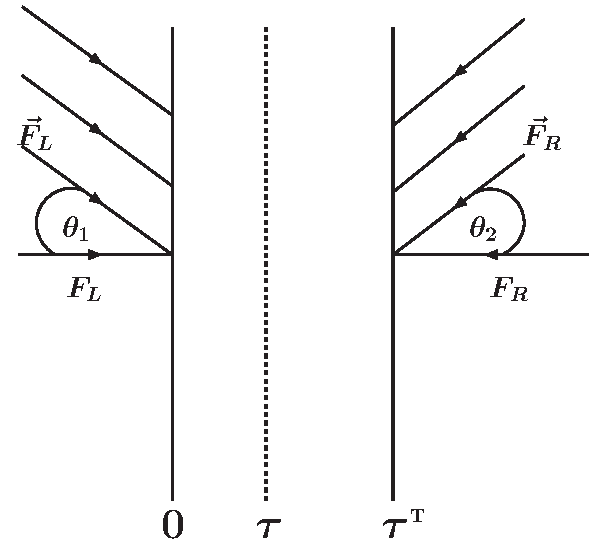
\includegraphics[width=0.35\hsize]{slab_dir}
  \hspace{1in}
  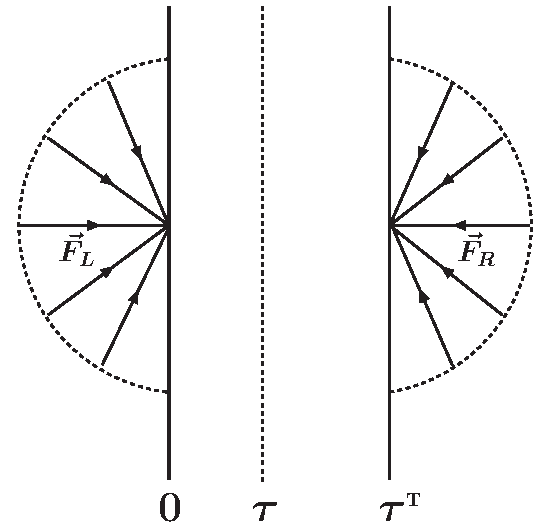
\includegraphics[width=0.35\hsize]{slab_iso}

  \caption{External heating of a slab. {\em Left}: Directional
    illumination from both sides. {\em Right}: Isotropic radiation on
    both sides. Note that the total flux vanishes in both cases
    whenever $\vec F_{\rm L} = \vec F_{\rm R}$.}
  \label{fig:slab}
\end{figure}
%%%%%%%%%%%%%%%%%%%%%%%%%%%%%%%%%%%%%%%%%%%%%%%%%%%%%%%%%%%%%%%%

\begin{itemize}

\item In the spherical case, the first flag is for a central
  source. For example,
\begin{verbatim}
            central = ON
\end{verbatim}
  is to be followed by input for spectral shape and strength of the
  central source. Afterwards comes the flag for the external
  radiation; for example
\begin{verbatim}
            external = OFF
\end{verbatim}
  ends the external radiation input in this case. \textbf{NOTE: Only
    one source of radiation, either internal or external, is allowed
    in the spherical case}

\item In the slab case, both isotropic radiation and parallel-ray
  illumination maintain the planar symmetry (see figure
  \ref{fig:slab}).  Therefore, the radiation angular distribution must
  be specified first, before its spectral shape and strength. Since
  the left-side radiation is always present, the first input is for
  its angular distribution:
\begin{verbatim}
       angular distribution = ISOTROPIC
\end{verbatim}
  for isotropic radiation or
\begin{verbatim}
       angular distribution = DIRECTIONAL
       illumination angle   = 60 degrees
\end{verbatim}
  for the parallel-rays case; because of numerical considerations,
  only $\theta \le$ 85\deg\ is allowed. Each case is to be followed by
  input for the spectral shape and strength of the left-side
  source. The optional right-side illumination is specified with an
  {\tt ON/OFF} flag. For example,
\begin{verbatim}
       right = OFF
\end{verbatim}
  indicates left-side illumination only, while additional radiation on
  the right is specified with
\begin{verbatim}
       right = ON
       angular distribution = DIRECTIONAL
       illumination angle   = 30 degrees
\end{verbatim}
  followed by input for the spectral shape and strength of the
  right-side source. You can mix the types of radiation, e.g.,
  directional on the left and isotropic on the right. Care must be
  taken to supply the proper illumination angle ($\le$ 85\deg) for
  each directional component.
\end{itemize}


Each external radiation component that is {\tt ON} must be
additionally specified by its spectral shape and strength. Next we
describe the input specifications for these properties.

\subsubsection{Spectral Shape of External Radiation}
\label{sec:type_raiation}
%
Because of scale invariance, the only property of the external
radiation that must be always specified is its spectral shape (see
\cite{IE97}). Six different selected input options are available in
\D. Three involve entry in analytical form: (1) a combination of
black-bodies, (2) an empirical expression devised by
Engelke~\cite{Engelk} and Marengo~\cite{Mareng}, and (3) broken power
law. The other three are for entry in numerical form as a separate
user-supplied input file which lists either (4) $\lambda F_\lambda$ (=
$\nu F_\nu$) or (5) $F_\lambda$, or (6) $F_\nu$ vs $\lambda$.  Here
$\lambda$ is wavelength in \mic\ and $\nu$ the corresponding
frequency, and $F_\lambda$ or $F_\nu$ is the external flux density in
arbitrary units. The detailed properties of the different options are
as follows:

\begin{itemize}
%
\item A combination of up to 10 black bodies, each described by a
  Planck function of a given temperature. Following the spectral flag,
  the number of black bodies is specified, followed by a list of the
  temperatures. When more then one black-body is specified, the
  temperature list must be followed by a list of the fractional
  contributions of the different components to the overall spectral
  shape.
%
  \begin{itemize}
%
  \item A single black body:
\begin{verbatim}
         Spectral Shape = BLACK_BODY
           Number of BB = 1
            Temperature = 10,000 K
\end{verbatim}

    Note that this could also be entered on a single line as

    \hskip 1in {\tt type = BLACK\_BODY , N = 1, T = 1E4}

  \item Two black bodies, e.g. a binary system, with the first one
    contributing 80\% of the total luminosity (note that the distance
    between the stars must be sufficiently small that the assumption
    of a central point source remain valid):
\begin{verbatim}
         Spectral Shape = BLACK_BODY
           Number of BB = 2
           Temperatures = 10,000, 2,500 K
           Luminosities = 4, 1
\end{verbatim}

  \end{itemize}

\item Engelke-Marengo function.  This expression improves upon the
  black-body description of cool star emission by incorporating
  empirical corrections for the main atmospheric effects. Engelke
  \cite{Engelk} found that changing the temperature argument of the
  Planck function from $T$ to $0.738T[1 + 79450/(\lambda T)]^{0.182}$
  adequately accounts for the spectral effect of H$^-$. Massimo
  Marengo \cite{Mareng} devised an additional empirical correction for
  molecular SiO absorption around 8 \mic, and has kindly made his
  results available to DUSTY. The selection of this combined
  Engelke-Marengo function requires as input the temperature and the
  relative (to the continuum) SiO absorption depth in~\%.

  \begin{itemize}
  \item Stellar spectrum parametrized with Engelke--Marengo function:
\begin{verbatim}
               Spectral Shape = ENGELKE_MARENGO
                  Temperature = 2500 K
         SiO absorption depth = 10 percents
\end{verbatim}
  \end{itemize}

\item Broken power law of the form
$$
\lambda F_\lambda \propto \cases{ 0 & $\phantom{\lambda(1) < {}}
  \lambda \le \lambda(1)$ \cr \lambda^{-k(1)} & $\lambda(1) < \lambda
  \le \lambda(2)$ \cr \lambda^{-k(2)} & $\lambda(2) < \lambda \le
  \lambda(3)$ \cr \vdots \cr \lambda^{-k(N)} & $\lambda(N) < \lambda
  \le \lambda(N + 1)$ \cr 0 & $\lambda(N+1) < \lambda$ \cr}
$$

In this case, after the option selection the number $N$ is entered,
followed by a list of the break points $\lambda(i)$, $i = 1\dots N+1$,
in \mic\ and a list of the power indices $k(i)$, $i = 1\dots N$.  It
is important to list the wavelengths $\lambda(i)$ in increasing order.

\begin{itemize}
\item A flat spectrum confined to the range 0.1--1.0 \mic:
\begin{verbatim}
         Spectral Shape = POWER_LAW
                      N = 1
                 lambda = 0.1, 1 micron
                      k = 0
\end{verbatim}
  All spectral points entered outside the range covered by \D's
  wavelength grid are ignored. If the input spectrum does not cover
  the entire wavelength range, all undefined points are assumed zero.
\end{itemize}

\item Stellar spectrum tabulated in a file. The filename for the input
  spectrum must be entered separately in the line following the
  numerical flag. This input file can optionally start with an
  arbitrary number of header lines, in which case they must be
  terminated by a line containing `$>$' in the first column. This
  header section is followed by a two-column tabulation of $\lambda$
  and $\lambda F_\lambda$, where $\lambda$ is in \mic\ and $\lambda
  F_\lambda$ is in arbitrary units. The number of entry data points is
  limited to a maximum of 10,000 but is otherwise arbitrary. The
  tabulation must be ordered in wavelength but the order can be either
  ascending or descending. If the shortest tabulated wavelength is
  longer than 0.01 \mic, the external flux is assumed to vanish at all
  shorter wavelengths.  If the longest tabulated wavelength is shorter
  than 3.6 cm, \D\ will extrapolate the rest of the spectrum with a
  Rayleigh-Jeans tail.

  \begin{itemize}
  \item Spectral Shape tabulated in file {\tt quasar.dat}:

    {\tt Spectral Shape = FILE\_LAMBDA\_F\_LAMBDA

      filename = data/quasar.dat}
  \end{itemize}

\item Stellar spectrum read from a file as in the previous option, but
  $F_\lambda$ is specified (in arbitrary units) instead of $\lambda
  F_\lambda$.

  \begin{itemize}
  \item Kurucz model atmosphere tabulated in file {\tt kurucz10.dat}:

    {\tt Spectral Shape = FILE\_F\_LAMBDA

      filename = data/kurucz10.dat}
  \end{itemize}

\item Stellar spectrum read from a file as in the previous option, but
  $F_\nu$ is specified (in arbitrary units) instead of $F_\lambda$.

  \begin{itemize}
  \item Spectral Shape tabulated in file {\tt quasar\_Fnu.dat}:

    {\tt Spectral Shape = FILE\_F\_NU

      filename = data/quasar\_Fnu.dat}
  \end{itemize}

\end{itemize}

Note that in the last three entry options, the filename for the input
spectrum must be entered separately in the line following the name
flag. Optionally, you may separate the flag line and the filename line
by an arbitrary number of lines that are either empty or commented out
(starting with {\tt `\%'}). The files quasar.dat, kurucz10.dat and
quasar\_Fnu.dat are distributed with DUSTY.


\subsubsection{Input Radiation Strength}
\label{sec:scaling_radiation}

There are five different ways to enter the scale of the input
radiation: (1) bolometric flux, (2) luminosity and distance, (3)
energy density, (4) dilution factor for black body radiation, and (5)
dust temperature on the illuminated boundary. Option (5) is applicable
only in the cases of central source for the spherical geometry and
left side illumination for the slab case. Examples of these options
follow.


\begin{itemize}
%
\item The input radiation strength can be specified by its bolometric
  flux, in $\rm W/m^2$, on the illuminated surface:
\begin{verbatim}
  Scale:    type of entry = FLUX
                       Fe = 2.6E4 W/m^2
\end{verbatim}
  In the spherical case this option can be used only for a central
  source, and {\tt Fe} is the illuminating flux on the inner
  boundary. In the slab case this option applies only for directional
  illumination, and {\tt Fe} is the flux entering from the left.
%
\item Alternatively, the heating flux can be specified by entering the
  source luminosity (in \Lo) and its distance (in cm) from the
  illuminated boundary:
\begin{verbatim}
 Scale:     type of entry = LUM_R1
                        L = 1.0E4       % Luminosity [in Lo] and
                        d = 3.43e14 cm  % distance [cm] from the source
\end{verbatim}
  This method is equivalent to the previous one with $F_{\rm e} =
  L/4\pi d^2$.
%
\item The heating radiation scale can be specified instead by its
  energy density at the illuminated boundary:
\begin{verbatim}
       Scale:     type of entry = ENERGY_DEN       % Energy density of
                              J = 2.5e-5 W/m^2     % the ext. radiation
\end{verbatim}
  This type of entry is essential in the case of isotropic
  illumination (in both the spherical and planar cases), where the
  flux is zero and the previous two methods cannot be used.
%
\item Since the black-body function carries an absolute scale, its
  flux level can be specified by a dilution factor ($\le 1$):
\begin{verbatim}
          Scale:   type of entry = DILUTN_FAC     % dilution factor
                               W = 1.0e-5
\end{verbatim}
  This type of entry can be used {\em only} when the spectral shape is
  a combination of one or more black-bodies. In the case of multiple
  components, the dilution factor refers to the black-body that
  carries the highest specified luminosity.
%
\item Thanks to scaling (\cite{IE97}), the dust temperature on the
  illuminated boundary can be specified instead of the heating
  radiation strength at that position. This option can be used only
  when there is one external source of heating radiation---a central
  source in the spherical case, left-side illumination in the slab
  case:
\begin{verbatim}
 Scale:     type of entry = T1        % Td at the illuminated boundary
                       Td = 1000  K
\end{verbatim}
  The input {\tt Td} is the dust temperature on the inner boundary of
  the spherical shell or the left surface of the slab. The
  corresponding external bolometric flux on the illuminated surface is
  computed by \D\ and listed in the default output file. In principle,
  different types of grains can have different temperatures at the
  same location. However, \D\ currently treats mixtures as single-type
  grains whose properties average the actual mix, therefore only one
  temperature is specified.
\end{itemize}

\subsection{Dust Properties}

Dust optical properties are described by the dust absorption and
scattering cross-sections, which depend on the grain size and
material. Currently, \D\ supports only single-type grains, namely, a
single size and chemical composition.  Grain mixtures can still be
treated, simulated by a single-type grain constructed from an
appropriate average.  This approximation will be removed in future
releases which will provide full treatment of grain mixtures.

\subsubsection{Chemical Composition}
\label{chemistry}

\D\ contains data for the optical properties of six common grain
types.  In models that utilize these standard properties, the only
input required is the fractional abundance of the relevant grains.  In
addition, optical properties for other grains can be supplied by the
user.  In this case, the user can either specify directly the
absorption and scattering coefficients or have \D\ calculate them from
provided index of refraction. The various alternatives are selected by
a flag, as follows:

\begin{itemize}

\item \D\ contains data for six common grain types: `warm' and `cold'
  silicates from Ossenkopff et al (\cite{Oss92}, {\tt Sil-Ow} and {\tt
    Sil-Oc}); silicates and graphite grains from Draine and Lee
  (\cite{DL84}, {\tt Sil-DL} and {\tt grf-DL}); amorphous carbon from
  Hanner (\cite{Hann88}, {\tt amC-Hn}); and SiC by P\`egouri\`e
  (\cite{Peg88}, {\tt SiC-Pg}).  Fractional number abundances must be
  entered for all these grain types, in the order listed.

  \begin{itemize}
  \item Mixture containing only dust grains with built-in data for
    optical properties:

\begin{verbatim}
   optical properties index = COMMON_GRAIN
   Abundances for supported grain types, standard ISM mixture:

       Sil-Ow  Sil-Oc  Sil-DL  grf-DL  amC-Hn   SiC-Pg
   x =  0.00    0.00    0.53    0.47    0.00     0.00
\end{verbatim}
  \end{itemize}
  The overall abundance normalization is arbitrary.  In this example,
  the silicate and graphite abundances could have been entered
  equivalently as 53 and 47, respectively.

\item With this option, the user can introduce up to ten additional
  grain types on top of those built-in.  First, the abundances of the
  six built-in types of grains are entered as in the previous
  option. Next, the number ($\le 10$) of additional grain types is
  entered, followed by the names of the data files, listed separately
  one per line, that contain the relevant optical properties. These
  properties are specified by the index of refraction, and \D\
  calculates the absorption and scattering coefficients using Mie
  theory.  Each data file can optionally start with an arbitrary
  number of header lines, in which case they must be terminated by a
  line containing `$>$' in the first column. This header section is
  followed by a three-column tabulation of wavelength in \mic, and
  real ({\tt n}) and imaginary ({\tt k}) parts of the index of
  refraction. The number of table entries is arbitrary, up to a
  maximum of 10,000. The tabulation must be ordered in wavelength but
  the order can be either ascending or descending. \D\ will linearly
  interpolate the data for {\tt n} and {\tt k} to its built-in
  wavelength grid. If the supplied data does not fully cover \D's
  wavelength range, the refraction index will be assumed constant in
  the unspecified range, with a value equal to the corresponding end
  point of the user tabulation. The file list should be followed by a
  list of abundances, entered in the same order as the names of the
  corresponding data files.

  \begin{itemize}
  \item Draine \& Lee graphite grains with three additional grain
    types whose {\tt n} and {\tt k} are provided by the user in data
    files {\tt amC-zb1.nk}, {\tt amC-zb2.nk} and {\tt amC-zb3.nk},
    distributed with DUSTY.  These files tabulate the most recent
    properties for amorphous carbon by Zubko et al \cite{Zubko}:

\begin{verbatim}
   Optical properties index = COMMON_AND_ADDL_GRAIN
   Abundances of built-in grain types:
         Sil-Ow  Sil-Oc  Sil-DL  grf-DL amC-Hn SiC-Pg
     x =  0.00    0.00    0.00    0.22   0.00  0.00

   Number of additional components = 3, properties listed in files
                     amC-zb1.nk
                     amC-zb2.nk
                     amC-zb3.nk
   Abundances for these components = 0.45, 0.10, 0.23
\end{verbatim}
  \end{itemize}

\item This option is similar to the previous one, only the absorption
  and scattering coefficients are tabulated instead of the complex
  index of refraction, so that the full optical properties are
  directly specified and there is no further calculation by \D.  The
  data filename is listed in the line following the option flag. This
  input file can optionally start with an arbitrary number of header
  lines, in which case they must be terminated by a line containing
  `$>$' in the first column. This header section is followed by a
  three-column tabulation of wavelength in \mic, absorption
  ($\sigma_{\rm abs}$) and scattering ($\sigma_{\rm sca}$) cross
  sections. Units for $\sigma_{\rm abs}$ and $\sigma_{\rm sca}$ are
  arbitrary, only their spectral variation is relevant. The number of
  entries is arbitrary, with a maximum of 10,000. The handling of the
  wavelength grid is the same as in the previous option.

  \begin{itemize}
  \item Absorption and scattering cross sections from the file {\tt
      ism-stnd.dat}, supplied with \D, listing the optical properties
    for the standard interstellar dust mixture:

\begin{verbatim}
    Optical properties index = TABULATED
    X-sections input file    = data/ism-stnd.dat
\end{verbatim}
  \end{itemize}

\end{itemize}

\D's distribution includes a library of data files with the complex
refractive indices of various compounds of common interest. This
library is described in appendix \ref{nklib}.

\subsubsection{Sublimation temperature}
\label{sec:sub_temp}

The dust sublimation temperature specifies the highest temperature at
which the dust grains can exist:
\begin{verbatim}
    Sublimation Temperature = 1500K
\end{verbatim}
If \D's solution includes dust at higher temperatures, these grains
are removed. When the specified input radiation strength (see
\S\ref{sec:scaling_radiation}) produces on the heated surface a dust
temperature higher than sublimation, it is changed such that that
temperature is the sublimation temperature. In addition \D\ will print
a warning message on the screen and in {\tt fname.out}. The Sections
\ref{sec:default_sph} (sphere) and \ref{sec:default_sph} (slab)
describe the file {\tt fname.out} in detail.

\subsubsection{Grain Size Distribution}

The grain size distribution must be specified only when the previous
option was set to {\tt COMMON\_GRAIN} or {\tt
  COMMON\_AND\_ADDL\_GRAIN}.  When the dust cross sections are read
from a file (previous option set at {\tt TABULATED}), this particular
option is skipped.

\D\ recognizes two distribution functions for grain sizes $n(a)$ ---
the MRN \cite{MRN77} power-law with sharp boundaries \eq{ n(a) \propto
  a^{-q} \qquad \hbox{for} \quad a_{\rm min} \le a \le a_{\rm max} }
and its modification by Kim, Martin and Hendry \cite{KMH94}, which
replaces the upper cutoff with a smooth exponential falloff \eq{ n(a)
  \propto a^{-q} e^{-a/a_0} \qquad \hbox{for} \quad a \ge a_{\rm min}}
\D\ contains the standard MRN parameters $q$ = 3.5, $a_{\rm min}$ =
0.005 \mic\ and $a_{\rm max}$ = 0.25 \mic\ as a built-in option.  In
addition, the user may select different cutoffs as well as power index
for both distributions.

\begin{itemize}

\item This is the standard MRN distribution.

  {\tt Size distribution = MRN}

  No input required other than the option flag.

\item Modified MRN distribution.  The option flag is followed by
  listing of the power index $q$, lower limit $a_{\rm min}$ and upper
  limit $a_{\rm max}$ in \mic.

  \begin{itemize}
  \item Standard MRN distribution can be entered with this option as:

    {\tt Size distribution = MODIFIED\_MRN

      q = 3.5, a(min) = 0.005 micron, a(max) = 0.25 micron}

  \item Single size grains with $a$ = 0.05 \mic:

\begin{verbatim}
     Size distribution = MODIFIED_MRN
                     q = 0 (it is irrelevant in this case)
                a(min) = 0.05 micron
                a(max) = 0.05 micron
\end{verbatim}
  \end{itemize}

\item KMH distribution \cite{KMH94}.  The option flag is followed by a
  list of the power index $q$, lower limit $a_{\rm min}$ and the
  characteristic size $a_0$ in \mic.

  \begin{itemize}
  \item Size distribution for grains in the dusty envelope around
    IRC+10216 as obtained by Jura \cite{Jura} and verified in \Ivezic\
    \& Elitzur \cite{IE96b}:

    {\tt Size distribution = KMH

      q = 3.5, a(min) = 0.005 micron, a0 = 0.2 micron}

  \end{itemize}
\end{itemize}


\subsection{Optical Depth}
\label{optical_depth} For a given set of the parameters specified
above, \D\ will generate up to 999 models with different overall
optical depths.  The list of optical depths can be specified in two
different ways.  \D\ can generate a grid of optical depths spaced
either linearly or logarithmically between two end-points specified in
the input.  Alternatively, an arbitrary list can be entered in a file.

\begin{itemize}

\item Optical depths covering a specified range in linear steps:
  Following the option selection, the fiducial wavelength $\lambda_0$
  (in \mic) of optical depth $\tau_0$ is entered.  The $\tau_0$ grid
  is then specified by its two ends and the number of points ($\le
  999$).

  \begin{itemize}
  \item Models with 2.2 \mic\ optical depths including all the
    integers from 1 to 100:

\begin{verbatim}
       tau grid = LINEAR
       lambda0  = 2.2 micron
       tau(min) = 1; tau(max) = 100
       number of models = 100
\end{verbatim}
  \end{itemize}

\item Same as the previous option, only the $\tau_0$ range is covered
  in logarithmic steps:

  \begin{itemize}
  \item Three models with visual optical depth $\tau_V$ = 0.1, 1 and
    10:
\begin{verbatim}
       tau grid = LOGARITHMIC
       lambda0  = 0.55 micron
       tau(min) = 0.1; tau(max) = 10
       number of models = 3
\end{verbatim}
  \end{itemize}

\item Optical depths list entered in a file: The file name is entered
  on a single line after the option selection. The supplied file can
  optionally start with an arbitrary number of header lines, in which
  case they must be terminated by a line containing `$>$' in the first
  column. This header section is followed by the fiducial wavelength
  $\lambda_0$, preceded by the equal sign, `='. The list of optical
  depths, one per line up to a maximum of 999 entries, is entered next
  in arbitrary order.  \D\ will sort and run it in increasing
  $\tau_0$.

  \begin{itemize}
  \item Optical depths from the file {\tt taugrid.txt}, supplied with
    the \D\ distribution:
\begin{verbatim}
       tau grid = USER_SUPPLIED  % grid supplied in file:
       data/taugrid.dat
\end{verbatim}
    The file {\tt taugrid.dat} is used in the sample input files {\tt
      slab2.inp} and {\tt sphere3.inp}.
  \end{itemize}
\end{itemize}

\subsection{Numerical Accuracy and Internal Bounds}
\label{numerics}

\D's accuracy is controlled by internal convergence criteria, as well
as the density of the wavelength and spatial grids employed in the
computations. The wavelength grid can be modified by users to meet
their specific needs (see \S\ref{F-Grid}) and it does not change
during execution. Flux conservation is controlled by the density of
the spatial grids. These are automatically generated and refined until
the fractional error of flux conservation at every grid point is less
than $q_{\rm acc}$, entered as
%
\begin{verbatim}
    accuracy for flux conservation = 0.1
\end{verbatim}
This accuracy is calculated from $(F_{\rm max} - F_{\rm min})/(F_{\rm
  max} + F_{\rm min})$, where $F_{\rm max}$ and $F_{\rm min}$ are the
two extremes of the computed flux values. Whenever \D\ calculates also
the density profile $\eta$ for spherical case, the numerical accuracy
of that calculation is controlled by the same $q_{\rm acc}$.

The recommended flux accuracy value of 10\% is entered in all the
sample input files. The accuracy level that can be accomplished is
related to the number of grid points and the model's overall optical
depth. If the desired accuracy is not achieved, finer grids are
generated automatically by \D. The maximum number of grid points is
bound by \D's array dimensions, which are controlled by the parameter
{\tt npy} whose default value is 120. This internal limit suffices to
ensure convergence at the 10\% level for most models with $\tau_V$
\la\ 1000.\footnote{Convergence and execution speed can be affected by
  the input radiation spectral shape. A hard spectrum heavily weighed
  toward short wavelengths, where the opacity is high, can have an
  effect similar to large \tV.} If higher levels of accuracy or larger
$\tau_V$ are needed, \D's internal limits on array sizes must be
expanded by increasing {\tt npy}, as described in \S\ref{Memory}.

\subsection{Output Control}

The final input entries control \D's output. All output and its
control is explained in the next section.


\section{Output: Sphere}
\label{sec:output_sph}

A typical \D\ run generates an enormous amount of information, and the
volume of output can easily get out of hand. To avoid that, \D's
default output is a single file that lists only minimal information
about the run, as described next. All other output is optional and
fully controlled by the user.

\subsection{Default Output for Sphere}
\label{sec:default_sph}

\D\ always produces the output file {\tt fname.out} for each model
input {\tt fname.inp}. In addition to a summary of the input
parameters, the default output file tabulates global properties for
each of the optical depths covered in the run.

The table's left column lists the sequential number {\tt \#\#\#} of
the model with the fiducial optical depth {\tt tau0} listed in the
next column.  Subsequent columns list quantities calculated by \D\ for
that {\tt tau0}:

\begin{list}{$\diamond$}{}
\item {\tt Psi/Psi0} -- Psi as defined by eq.14 in IE97 with optically
  thin value Psi0= 6.06E+00
\item {\tt Fi} -- the bolometric flux, in $\rm W\ m^{-2}$, at the
  inner radius $y = 1$. Only the central source contributes to {\tt
    Fi}; the diffuse flux vanishes at $y = 1$ under the point source
  assumption and the external radiation field carries no flux because
  it is isotropic. The bolometric flux emerging from the spherical
  distribution is {\tt F1/$Y^2$}.

  Any measure of the shell dimension is irrelevant to the radiative
  transfer problem and thus not part of \D's calculations.  Still, the
  shell size can be of considerable interest in many applications. For
  convenience, the next three output items list different measures of
  the shell size expressed in terms of redundant quantities such as
  the luminosity:

\item {\tt r1(cm)} -- the shell inner radius. If the heating radiation
  strength is specified through option {\tt T1} (see
  \S\ref{sec:scaling_radiation}) then {\tt r1} is the radius where
  this is the dust temperature. This radius scales in proportion to
  $L^{1/2}$, where $L$ is the luminosity. The tabulated value
  corresponds to $L$ = \E4~\Lo.

\item {\tt r1/rc} -- where {\tt rc} is the radius of the central
  source.  This quantity scales in proportion to $(T_e/T_1)^2$, where
  $T_e$ is the external radiation effective temperature.  The listed
  value is for $T_e = 10,000$ K with two exceptions: when the spectral
  shape of the external radiation is the Planck or Engelke-Marengo
  function, the arguments of those functions are used for $T_e$.

\item {\tt theta1} -- the angular size, in arcsec, of the shell inner
  diameter.  This angle depends on the observer's position and scales
  in proportion to $F_{\rm obs}^{1/2}$, where $F_{\rm obs}$ is the
  observed bolometric flux.  The tabulated value corresponds to
  $F_{\rm obs} = \E{-6}\ \rm W\ m^{-2}$.

\item {\tt T1} -- the dust temperature, in K, at the envelope's inner
  boundary. When the specified input radiation strength (see
  \S\ref{sec:scaling_radiation}) produces a temperature in excess of
  the sublimation temperature {\tt Tsub}, it is changed such that {\tt
    T1 = Tsub} and \D\ will print a warning message.

\item {\tt Td} -- the dust temperature, in K, at the envelope's outer
  boundary $(y = Y)$.

\item {\tt RPr(1)} -- The ratio of radiation pressure to gravitational
  force at the inner boundary. Both forces are per unit volume: \eq{
    {\Frad\over\Fgrav} = {1\over4\pi Gcm} \cdot{L\over
      M}\cdot{n_d\sigma_V\over n_H}\, \int\!Q_\lambda
    f_\lambda\,d\lambda } Here $m$ is the mass of a hydrogen atom,
  $f_\lambda = F_\lambda/\int F_\lambda d\lambda$ is the local
  spectral shape, $n_d$ the dust number density and $n_H$ the number
  density of hydrogen nuclei.  This expression holds only if the gas
  and dust are fully collisionally coupled. The tabulated value is for
  the standard Galactic value $n_d\sigma_V/n_H = 5\cdot\E{-22}$
  cm$^{-2}$ and for $L/M$ = \E4 \Lo/\Mo.

\item {\tt err} -- the numerical accuracy, in {\tt \%}, achieved in
  the run.  Specifically, if $r$ is the ratio of smallest to largest
  bolometric fluxes in the shell (after accounting for radial dilution
  in a centrally heated spherical shell), then the error is $(1 -
  r)/(1 + r)$. Errors smaller than 1\% are listed as zero.

\end{list}
When the density distribution is derived from a hydrodynamics
calculation for AGB winds (\S\ref{winds}), three more columns are
added to {\tt fname.out}:
\begin{list}{$\diamond$}{}
\item {\tt Mdot} -- the mass loss rate in \Mo\ $\rm yr^{-1}$.  This
  quantity has \about\ 30\% inherent uncertainty because varying the
  gravitational correction from 0 up to 50\% has no discernible effect
  on the observed spectrum.

\item {\tt Ve} -- the terminal outflow velocity in \kms. The provided
  solutions apply only if this velocity exceeds 5 \kms.  {\tt Ve} is
  subject to the same inherent uncertainty as {\tt Mdot}.
\item {\tt M$>$} -- an upper limit in \Mo\ on the stellar mass $M$.
  The effect of gravity is negligible as long as $M$ is less than
  0.5{\tt *M$>$} and the density profile is then practically
  independent of $M$.

\end{list}
These quantities posses general scaling properties in terms of the
luminosity $L$, gas-to-dust mass ratio $r_{\rm gd}$ and dust grain
bulk density $\rho_s$ \cite{EI01, IE10}; the tabulations are for $L$ =
\E4\ \Lo, $r_{\rm gd} = 200$ and $\rho_s = 3\ \rm g~cm^{-3}$. There is
a slight complication with these tabulations when the dust optical
properties are entered using {\tt optical properties = 3} (\S
\ref{chemistry}). With this option, the scattering and absorption
cross sections are entered in a file, tabulated using arbitrary units
since only their spectral shape is relevant for the solution of the
radiative transfer problem. However, the conversion to mass-loss rate
requires also the grain size, and this quantity is not specified when
{\tt optical properties = 3} is used.  \D\ assumes that the entered
values correspond to $\sigma/V$, the cross section per grain volume in
$\mic^{-1}$.  If that is not the case, in the scaling relations
$r_{\rm gd}$ must be replaced with $r_{\rm gd}V/\sigma$.

Finally, \D\ assumes that the external radiation originates in a
central point source. This assumption can be tested with eqs.\ (27)
and (28) of \cite{IE97} which give expressions for the central source
angular size and occultation effect. From these it follows that the
error introduced by the point-source assumption is no worse than 6\%
whenever \eq{\label{Tmin} T_e > 2\times\max[T_1,
  (F_{e1}/\sigma)^{1/4}]} where $T_e$ is the effective temperature of
the central source and $F_{e1}$ is its flux at the shell inner
boundary; note again that with the point source assumption, {\tt F1} =
$F_{e1}$. Thanks to scaling, \Te\ need not be specified and is
entirely arbitrary as far as \D\ is concerned. However, compliance
with the point-source assumption implies that the output is meaningful
only for sources whose effective temperature obeys eq.\
\ref{Tmin}. For assistance with this requirement, {\tt fname.out}
lists the lower bound on $T_e$ obtained from this relation for
optically thin sources. Since $F_{e1}$ decreases with optical depth
when {\tt T1} is specified as input (see \cite{IE97}), the listed
bound ensures compliance for all the models in the series. However, in
optically thick cases $F_{e1}$ may become so small that the listed
bound will greatly exceed the actual limit from eq.\ \ref{Tmin}. In
those cases, the true bounds can be obtained, if desired, from eq.\
\ref{Tmin} and the model tabulated {\tt F1}.

Black-body emission provides an absolute upper bound on the intensity
of any thermal source. Therefore, input radiation whose spectral shape
is the Planck function at temperature $T$ is subject to the limit $T_e
\le T$ even though $T_e$ is arbitrary in principle. In such cases $T$
must comply with eq.\ \ref{Tmin}, otherwise \D's output is suspect and
in fact could be meaningless.  \D\ issues a stern warning after the
tabulation line of any model with input spectral shape that is either
the Planck or Engelke-Marengo function whose temperature violates eq.\
\ref{Tmin}.




\subsection{Optional Output for Sphere}
\label{sec:optional_sph}

In addition to the default output, the user can obtain numerous
tabulations of spectra, imaging profiles and radial distributions of
various quantities of interest for each of the optical depths included
in the run. This additional output is controlled through flags entered
at the end of the input file {\tt fname.inp} that turn on and off the
optional tabulations.  Setting all flags to 0, as in {\tt sphere1.inp}
and {\tt slab1.inp}, suppresses all optional tabulations and results
in minimal output. A non-zero output flag triggers the production of
corresponding output, occasionally requiring additional input.
Further user control is provided by the value of the output flag. When
a certain flag is set to 1, the corresponding output is listed in a
single file that contains the tabulations for all the optical depth
solutions. Setting the flag to 2 splits the output, when appropriate,
tabulating the solution for each optical depth in its own separate
file. This may make it more convenient for plotting purposes, for
example, at the price of many small files.  A few flags can also be
set to 3, splitting the output even further.

Each of the following subsections describes in detail the optional
tabulations triggered by one of the output flags and any additional
input it may require.  Appendix \ref{summary} summarizes all the
output flags and the corresponding output files they trigger, and can
be used for quick reference.


\subsubsection {Detailed spectra for each model}
\label{sec:detail_sph}

The next output flag triggers listing of detailed spectra for each
model in the run.  Setting this flag to 1 produces tables for the
emerging spectra of all models in the single output file {\tt
  fname.stb}.  Setting the flag to 2 places each table in its own
separate file, where file {\tt fname.s\#\#\#} contains the tabulation
for model number {\tt \#\#\#} in the optical depth sequence listed in
the default output file (\S~\ref{sec:default_sph}).

Spectra are tabulated in terms of their spectral shapes $f(\lambda) =
\lambda F_\lambda/\int\!F_\lambda d\lambda$, where $F_\lambda$ is the
relevant flux.  The corresponding scale $F = \int\!F_\lambda d\lambda$
in [W/m$^2$] is listed in the table's first row (specified with a
wavelength of $-1$), followed by listing of $f_\lambda$. Values
smaller than \E{-20} are listed as 0. In addition to the emerging
spectrum, the table for each model also lists separately the
contributions of various components to the overall flux, the spectral
shape of the input radiation, and the wavelength dependence of the
total optical depth. The tabulated quantities are :

\begin{list}{$\diamond$}{}
\item {\tt lambda} -- the wavelength in \mic
\item {\tt fTot} -- the spectral shape of the total emerging flux
  % $f(\lambda) = \lambda F_\lambda/\int\!F_\lambda d\lambda$.  Values
  % smaller than \E{-20} are listed as 0.
\item{\tt xAtt} -- fractional contribution of the attenuated input
  radiation to {\tt fTot}
\item{\tt xDs} -- fractional contribution of the scattered radiation
  to {\tt fTot}
\item{\tt xDe} -- fractional contribution of the dust emission to {\tt
    fTot}
\item{\tt fInp} -- the spectral shape of the input (unattenuated)
  radiation
\item{\tt tauT} -- overall optical depth at wavelength {\tt lambda}
\item{\tt albedo} -- the albedo at wavelength {\tt lambda}
\end{list}

\subsubsection{Images at specified wavelengths}
\label{sec:images_sph}

The surface brightness is a luminosity-independent self-similar
distribution \cite{IE96a} of $b/r_1$, the impact parameter scaled by
the envelope inner radius (fig. \ref{impact parameter}); note that
$r_1$ is listed in the default output file (\S\ref{sec:default_sph})
for a source luminosity \E4~\Lo. \D\ can produce maps of the surface
brightness at up to 20 wavelengths, specified in the input
file. Setting the option flag to 1 produces imaging tabulations for
all the models of the run in the single output file {\tt fname.itb},
setting the flag to 2 puts the table for model number {\tt \#\#\#} in
its separate file {\tt fname.i\#\#\#}.

\begin{figure}[ht]
  \centering
  % 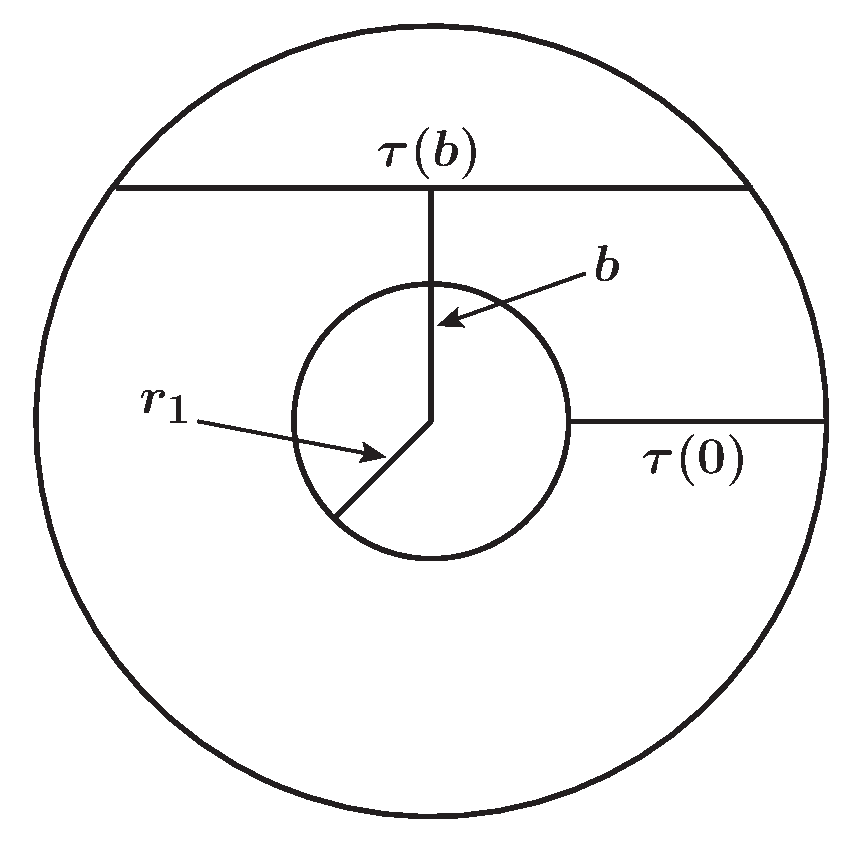
\includegraphics[width=0.40\hsize]{figure1.eps}
  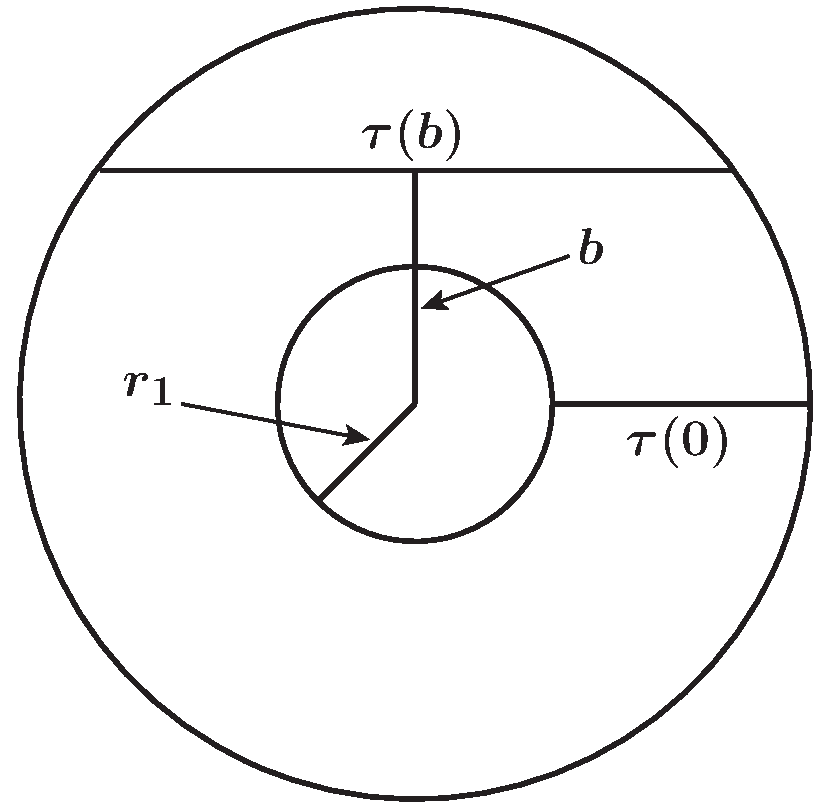
\includegraphics[width=0.40\hsize]{sphere}
  \caption{Notation for imaging output.}
  \label{impact parameter}
\end{figure}

Following the option selection flag, the number ($\le 20$) of desired
wavelengths is entered first, followed by a list of these wavelengths
in \mic.

\begin{itemize}
\item Example of additional input data required in {\tt fname.inp} for
  imaging output:
\begin{verbatim}
 imaging tables (all models in one file) = 1
 number of wavelengths = 8
 wavelengths = 0.55, 1.0, 2.2, 4, 10, 50, 100, 1000  micron
\end{verbatim}
\end{itemize}
Whenever a specified wavelength is not part of \D's grid, the
corresponding image is obtained by linear interpolation from the
neighboring wavelengths in the grid.  If the nearest wavelengths are
not sufficiently close, the interpolation errors can be
substantial. For accurate modeling, all wavelengths specified for
imaging should be part of the grid, modifying it if necessary (see
\S\ref{F-Grid}).

Each map is tabulated with a single header line as follows:
\begin{list}{$\diamond$}{}
\item{\tt b} $= b/r_1$, where $b$ is the impact parameter.
\item {\tt t(b)} = $\tau(\tt b)/\tau(0)$, where $\tau(\tt b)$ is the
  overall optical depth along a path with impact parameter {\tt
    b}. Note that $\tau(0)$ is simply the overall radial optical depth
  {\tt tauT}, listed in the file {\tt fname.s\#\#\#} (\S
  \ref{sec:detail_sph}), and that {\tt t(b)} doubles its value across
  the shell once the impact parameter exceeds the stellar radius.
\item The intensity, in Jy arcsec$^{-2}$, at each of the wavelengths
  listed in the header line.
\end{list}

A typical image contains a narrow central spike of width $b_c =
2r_c/r_1$, where $r_c$ is the radius of the central source
\cite{IE96a}.  Since this feature is unresolved in most observations,
it is usually of limited interest.  This spike is the only feature of
the emerging intensity that depends on the effective temperature \Te\
of the central source, which is irrelevant to \D's calculations. The
width of the spike scales in proportion to $T_e^{-2}$, its height in
proportion to $T_e^4$. The listed value is for $T_e = 10,000$ K with
two exceptions: when the spectral shape of the external radiation is
the Planck or Engelke-Marengo function, the arguments of those
functions are used for $T_e$.

\subsubsection{Radial profiles for each model}
\label{sec:radial_sph}

The next option flag triggers tabulations of the radial profiles of
the density, optical depth and dust temperature. Setting the flag to 1
produces tabulations for all the models of the run in the single
output file {\tt fname.rtb}, setting the flag to 2 places the table
for model number {\tt \#\#\#} in its own separate file {\tt
  fname.r\#\#\#}. The tabulated quantities are:

\begin{list}{$\diamond$}{}
\item{\tt y} -- dimensionless radius
\item{\tt eta} -- the dimensionless, normalized radial density profile
  (\S \ref{sec:eta})
\item {\tt t} -- radial profile of the optical depth variation.  At
  any wavelength $\lambda$, the optical depth at radius $y$ measured
  from the inner boundary is {\tt t*tauT}, where {\tt tauT} is the
  overall optical depth at that wavelength, tabulated in the file {\tt
    fname.s\#\#\#} (\S \ref{sec:detail_sph}).

\item{\tt tauF} -- radial profile of the flux-averaged optical depth
\item {\tt epsilon} -- the fraction of grain heating due to the
  contribution of the envelope to the radiation field (see
  \cite{IE97}).
\item{\tt RPr} -- radial profile of the ratio of radiation pressure to
  gravitational force normalized to the value of the ratio at the
  inner boundary, {\tt RPr$(y = 1)$}. The inner boundary value is
  listed in the default file {\tt fname.out} (\S
  \ref{sec:default_sph}).
\item{\tt Td} -- radial profile of the dust temperature

\end{list}
The radial profiles {\tt eta}$(y)$ and {\tt t}$(y)$ determine also the
radial runs of gas density and column density once a dust-to-gas ratio
is assumed; the standard conversion is that the hydrogen column
associated with dust optical depth \tV\ is $N_{\rm H} = 2\cdot\E{21}$
\tV\ cm$^{-2}$. Then the radial profiles of gas column and volume
densities are
\begin{equation}\label{eq:profiles}
  N_{\rm H}(y) = N_{\rm H}\times{\tt t}(y), \qquad
  n_{\rm H}(y) = (N_{\rm H}/r_1)\times{\tt eta}(y)
\end{equation}
In the case of dynamical calculation with {\tt density type = 3} for
AGB stars (\S\ref{winds}), the following additional profiles are
tabulated:

\begin{list}{$\diamond$}{}
\item {\tt u} -- the dimensionless radial velocity profile normalized
  to the terminal velocity {\tt Ve}, which is tabulated for the
  corresponding overall optical depth in file {\tt fname.out} (\S
  \ref{sec:default_sph}).
\item {\tt drift} -- the radial variation of $v_{\rm g}/v_{\rm d}$,
  the velocity ratio of the gas and dust components of the envelope.
  This quantity measures the relative decrease in dust opacity due to
  dust drift.

\end{list}

\subsubsection{Detailed Run-time messages}
\label{sec:error_sph}

In case of an error, the default output file issues a
warning. Optionally, additional, more detailed run-time error messages
can be produced and might prove useful in tracing the program's
progress in case of a failure. Setting the corresponding flag to 1
produces messages for all the models in the single output file {\tt
  fname.mtb}, setting the flag to 2 puts the messages for model number
{\tt \#\#\#} in its own separate file {\tt fname.m\#\#\#}.


\section{Output: Slab}
\label{sec:output_slb}

\subsection{Default Output for Slab}
\label{sec:default_slb}

\D\ always produces the output file {\tt fname.out} for each model
input {\tt fname.inp}. In addition to a summary of the input
parameters, the default output file tabulates global properties for
each of the optical depths covered in the run.

The table's left column lists the sequential number {\tt \#\#\#} of
the model with the fiducial optical depth {\tt tau0} listed in the
next column.  Subsequent columns list quantities calculated by \D\ for
that {\tt tau0}:


\begin{list}{$\diamond$}{}
\item{\tt Psi/Psi0} -- Psi as defined by eq.14 in IE97 with optically
  thin value Psi0= 4.78E+01
\item{\tt FiL} -- input bolometric flux, in $\rm W\,m^{-2}$, of the
  left-side source at the slab left boundary.
\item{\tt FiR} -- input bolometric flux, in $\rm W\,m^{-2}$, of the
  right-side source at the slab left boundary.
\item{\tt FbolL} -- bolometric flux, in $\rm W\,m^{-2}$, at the left
  slab boundary.
\item{\tt FbolR} -- bolometric flux, in $\rm W\,m^{-2}$, at the right
  slab boundary.
\item{\tt r1(cm)} -- the distance at which a point source with
  luminosity \E4 \Lo\ produces the bolometric flux $F_{e1}$.
\item {\tt TdL(K)} -- the dust temperature at the slab left
  boundary. When the specified input radiation strength (see
  \S\ref{sec:scaling_radiation}) produces a temperature in excess of
  the sublimation temperature {\tt Tsub}, it is changed such that {\tt
    TdL = Tsub} and \D\ will print a warning message.
\item {\tt TdR(K)} -- the dust temperature at the slab right boundary.
  See previous item for values in excess of {\tt Tsub}.
\item {\tt RPr(1)} -- The ratio of radiation pressure to gravitational
  force at the left boundary. Both forces are per unit volume: \eq{
    {\Frad\over\Fgrav} = {1\over4\pi Gcm} \cdot{L\over M}
    \cdot{n_d\sigma_V\over n_H}\, \int\!Q_\lambda f_\lambda\,d\lambda
  } Here $m$ is the mass of a hydrogen atom, $f_\lambda =
  F_\lambda/\int F_\lambda d\lambda$ is the local spectral shape,
  $n_d$ the dust number density and $n_H$ the number density of
  hydrogen nuclei.  This expression holds only if the gas and dust are
  fully collisionally coupled. The tabulated value is for the standard
  Galactic ratio $n_d\sigma_V/n_H = 5\cdot\E{-22}$ cm$^{-2}$ and for
  $L/M$ = \E4 \Lo/\Mo.
\item{\tt err} -- the flux conservation error, defined as in the
  spherical case.

\end{list}

\bigskip \D's distribution contains three sample input files, {\tt
  slab1.inp}, {\tt slab2.inp} and {\tt slab3.inp}, which can be used
as templates for the slab geometry. The output generated with {\tt
  slab1.inp} is shown in appendix \ref{slab1}.

\subsection{Optional Output for Slab}
\label{sec:optional_slb}

\subsubsection{Detailed spectra for each model }
\label{sec:detail_slb}

The next output flag triggers listing of detailed spectra for each
model in the run.  Setting this flag to 1 producerrs tables for the
emerging spectra of all models in the single output file {\tt
  fname.stb}.  Setting the flag to 2 places each table in its own
separate file, where file {\tt fname.s\#\#\#} contains the tabulation
for model number {\tt \#\#\#} in the optical depth sequence listed in
the default output file (\S\ref{sec:default_slb}).

The structure of the output is the same as for the sphere
(Sect.~\ref{sec:detail_sph}). Spectra are tabulated in terms of their
spectral shapes $f(\lambda) = \lambda F_\lambda/\int\!F_\lambda
d\lambda$, where $F_\lambda$ is the relevant flux. The corresponding
scale $F = \int\!F_\lambda d\lambda$ in [W/m$^2$] is listed in the
table's first row (specified with a wavelength of $-1$), followed by
listing of $f_\lambda$.  Values smaller than \E{-20} are listed as
0. In addition to the emerging spectrum, the table for each model also
lists separately the contributions of various components to the
overall flux, the spectral shape of the input radiation, and the
wavelength dependence of the total optical depth.  The tabulated
quantities are :
%
%
% In addition to the emerging spectrum for both sides of the slab, the
% table for each model also lists separately the contributions of
% various components to the overall flux, the spectral shape of the
% input radiation, and the wavelength dependence of the total optical
% depth. The structure of the output is the same as for the sphere
% case (Sect.~\ref{sec:detail_sph}). All emerging spectra
% (xAtt,xDs,xDs,finp) are of the form $\lambda f_{\lambda} F$. The
% scale $F$ in [W/m$^2$] is listed in the first line specified with a
% wavelength of $-1$. In the following rows the shape is listed as
% $\lambda f_\lambda$ .  The tabulated quantities are :
%
\begin{list}{$\diamond$}{}
\item {\tt lambda} -- the wavelength in \mic
\item {\tt fRight/fLeft} -- the spectral shape of the total flux
  emerging from the right/left side of the slab.
%
  % flux $f(\lambda) = \lambda F_\lambda/\int\!F_\lambda d\lambda$
  % from the right/left side of the slab.  Values smaller than \E{-20}
  % are listed as 0.
\item{\tt xAtt} -- fractional contribution of the attenuated input
  radiation to {\tt fTot}
\item{\tt xDs} -- fractional contribution of the scattered radiation
  to {\tt fTot}
\item{\tt xDe} -- fractional contribution of the dust emission to {\tt
    fTot}
\item{\tt fInp\_L/fInp\_R} -- the spectral shape of the input
  (unattenuated) radiation from left/right side of the slab
\item{\tt tauT} -- overall optical depth at wavelength {\tt lambda}
\item{\tt albedo} -- the albedo at wavelength {\tt lambda}
\end{list}

\subsubsection{Intensities for each model }
\label{sec:inten_slb}

The next output flag triggers listing of the intensity for user
specified angles for each model in the run.  Setting this flag to 1
produces tables for the emerging spectra of all models in the single
output file {\tt fname.itb}.  Setting the flag to 2 places each table
in its own separate file, where file {\tt fname.i\#\#\#} contains the
tabulation for model number {\tt \#\#\#} in the optical depth sequence
listed in the default output file (\S\ref{sec:default_slb}).

After triggering the the intensities file with the output flag the
angle grid has to be specified. First the type of the grid either
linear (1) or logarithmic (2). The next input is the minimum angle
followed by the maximum angle and the steppsize inbetween.

\begin{verbatim}
  intensities at specified angles;     fname.i### = 2
  angletype = 1 (linear)
  theta_min = 0 theta_max = 80 stepp = 5
\end{verbatim}

The tabulated quantities are :
\begin{list}{$\diamond$}{}
\item {\tt lambda} -- the wavelength in \mic
\item {\tt angle} -- the transmitted Intensity as $I(\theta)
  cos(\theta)$ in [W/sr]
\end{list}


\subsubsection{Spatial Profiles}
\label{sec:spatial_slb}

The output for spatial profiles is similar to the spherical case. The
radial distance {\tt y} and density profile {\tt eta} are removed. The
relative distance in optical depth from the left boundary, {\tt t},
becomes the running variable, and the tabulations of {\tt tauF}, {\tt
  epsilon}, {\tt Td} and {\tt RPr} are the same (see
\ref{sec:radial_sph}).



\subsubsection{Detailed Run-time messages}
\label{sec:error_slb}

These messages are triggered in the same way as in the spherical case
(see \S\ref{sec:error_sph}).


\section{User Control of \D}
\label{sec:user_control}

\D\ allows the user control of some of its inner working through
tinkering with actual code statements that control the spatial and
spectral grids. The appropriate statements were placed in the file
{\tt userpar.inc} separate from the main {\tt dusty.f}, and are
imbedded during compilation by the FORTRAN statement {\tt INCLUDE};
note that {\tt userpar.inc} \emph{must always stay with the source
  code in the same directory}. After modifying statements in {\tt
  userpar.inc} , \D\ must be recompiled to enable the changes.

\subsection{Array Sizes for Spatial Grid}
\label{Memory}

The maximum size of \D's spatial grid is bound by array
dimensions. These are controlled by the parameter {\tt npY} which sets
the limit on the number of radial points.  The default value of 40
must be decreased when \D\ is run on machines that lack sufficient
memory (see \S\ref{sec:Introduction}) and increased when \D\ fails to
achieve the prescribed accuracy (see \S\ref{numerics}). This parameter
is defined in {\tt userpar.inc} via
\begin{verbatim}
      PARAMETER (npY=512)
\end{verbatim}
To modify {\tt npY} simply open {\tt userpar.inc}, change the number
40 to the desired value, save your change and recompile.  That's all.
Every other modification follows a similar procedure. Since \D's
memory requirements vary roughly as the second power of {\tt npY}, the
maximum value that can be accommodated on any given machine is
determined by the system memory.

The parameter {\tt npY} defines also the size {\tt npP} of the grid
used in angular integrations.  In the case of planar geometry \D\ uses
analytic expressions for these integrations.  Since this grid becomes
redundant, {\tt npP} can be set to unity, allowing a larger maximum
{\tt npY}.  The procedure is described in {\tt userpar.inc}.

\subsection{Wavelength Grid} \label{F-Grid}

\D's wavelength grid is used both in the internal calculations and for
the output of all wavelength dependent quantities. The number of grid
points is set in {\tt userpar.inc} by the parameter {\tt npL}. The
grid itself is read from the file {\tt lambda\_grid.dat}, which
\emph{must always stay in the directory {\tt data}}.  This file starts
with an arbitrary number of header lines, the beginning of the
wavelength list is signaled by an entry for the number of grid
points. This number must be equal to {\tt npL} entered in {\tt
  userpar.inc} and to the actual number of entries in the list.

The grid supplied with \D\ contains 125 points from 0.01 to
$3.6\times10^{4}$ \mic.  The short wavelength boundary is to ensure
adequate coverage of input radiation from an O star, for example,
which peaks at 0.1 \mic.  Potential effects on the grain material by
such hard radiation are not included in \D.  The long wavelength end
is to ensure adequate coverage at all wavelengths where dust emission
is potentially significant. Wavelengths can be added and removed
provided the following rules are obeyed:
\begin{itemize}
\item Wavelengths are specified in \mic.
\item The shortest wavelength must be 0.01 \mic, the longest
  $3.6\times10^{4}$ \mic.
\item The ratio of each consecutive pair must be $\le$ 1.5.
\end{itemize}
The order of entries is arbitrary, \D\ sorts them in increasing
wavelength and the sorted list is used for all internal calculations
and output.  This provides a simple, convenient method for increasing
the resolution at selected spectral regions: just add points at the
end of the supplied grid until the desired resolution is attained.
Make sure you update both entries of {\tt npL} and recompile \D.

In practice, tinkering with the wavelength grid should be reserved for
adding spectral features. Specifying the optical properties of the
grains at a resolution coarser than that of the wavelength grid
defeats the purpose of adding grid points. The optical properties of
grains supported by \D\ are listed on the default wavelength grid.
Therefore, modeling of very narrow features requires both the entry of
a finer grid in {\tt lambda\_grid.dat} and the input of user-supplied
optical properties (see \S\ref{chemistry}) defined on that same grid.


% \newpage

\addcontentsline{toc}{section}{\bf Appendices}
\begin{appendix}
  \section*{\sc Appendices}
  % \addtocontents{toc}%{\break \vfil}


  \section{Output Summary}
  \label{summary}

  \D's default output is the file {\tt fname.out}, described in
  \S\ref{sec:default_sph} (sphere) and \S\ref{sec:default_slb}
  (slab). Additional output is optionally produced through selection
  flags, summarized in the following table.  The second column lists
  the section number where a detailed description of the corresponding
  output is provided.

  \begin{table}[htbp]
    \begin{center}
      \renewcommand{\arraystretch}{1.3}

\caption{\hfil Summary of all Output Options}\label{Options Table}
\centerline{} \renewcommand{\arraystretch}{1.3}
\begin{tabular}{|l|r||c|c|c|} \hline \multicolumn{1}{|c|}{Output
    Listing} & \multicolumn{1}{c||}{\S} & \multicolumn{3}{|c|}{Output
    File Triggered by Flag} \\ \cline{3-5} & & 1 & 2 & 3 \\ \hline
  {\bf Sphere} & & & &\\
  \hline
  Detailed spectra, each model     & \ref{sec:detail_sph} & {\tt fname.stb} & {\tt fname.s\#\#\#} & {\tt fname.s\#\#\#} \\
  \hline
  Images                           & \ref{sec:images_sph} & {\tt fname.itb} & {\tt fname.i\#\#\#} & {\tt fname.i\#\#\#} \\
  \hline
  Radial profiles                  & \ref{sec:radial_sph} & {\tt fname.rtb} & {\tt fname.r\#\#\#} &  \\
  \hline
  Error messages                   & \ref{sec:error_sph} & {\tt fname.mtb} & {\tt fname.m\#\#\#} &  \\
  \hline
  {\bf Slab} & & & &\\
  \hline
  Detailed spectra, each model     & \ref{sec:detail_slb} & {\tt fname.stb} & {\tt fname.s\#\#\#} & {\tt fname.s\#\#\#} \\
  \hline
  Intensities                      & \ref{sec:inten_slb}  & {\tt fname.itb} & {\tt fname.i\#\#\#} & {\tt fname.i\#\#\#} \\
  \hline
  Spatial profiles                 & \ref{sec:spatial_slb} & {\tt fname.rtb} & {\tt fname.r\#\#\#} &  \\
  \hline
  Error messages                   & \ref{sec:error_slb}  & {\tt fname.mtb} & {\tt fname.m\#\#\#} &  \\
  \hline
\end{tabular}
\end{center}
\end{table}


\section{Pitfalls, Real and Imaginary} \label{pitfalls}

This appendix provides a central depository of potential programming
and numerical problems. Some were already mentioned in the text and
are repeated here for completeness.

\begin{itemize}
\item FORTRAN requires termination of input records with a carriage
  return.  Make sure you press the ``Enter" key whenever you enter a
  filename in the last line of {\tt dusty.mas}.

\item In preparing input files, the following two rules must be
  carefully observed: (1) all required input entries must be
  specified, and in the correct order; (2) the equal sign, `=', must
  be entered only as a flag to numerical input. When either rule is
  violated and \D\ reaches the end of the input file while looking for
  additional input, you will obtain the error message:
\begin{verbatim}
     ****TERMINATED. EOF reached by RDINP while looking for input.
     *** Last line read:
\end{verbatim}
  This message is a clear sign that the input is out of order.

  % \newpage

\item On occasion, when the execution results in a segmentation fault
  under Linux or MacOS, increasing the stacksize of the console may
  solve the problem. This can be done as follows:
  \begin{quote}
    for a bash shell: {\tt ulimit -s unlimited}

    for a tcsh shell: {\tt limit stacksize unlimited}
  \end{quote}

\end{itemize}

% \vspace {1cm}

\newpage

\section{Sample Output File: {\tt sphere1.out}}
\label{sphere1}

\begin{verbatim}
 ===========================
  Output from program dusty
  version: 4.00
 ===========================

  Input parameters from file:
  examples/sphere1/sphere1.inp
* ----------------------------------------------------------------------
* NOTES:
* Sample input file (sphere1.inp)
* Spherical dust distribution with
* constant density profile
* heated by external radiation with a Black Body of 5000K
* for composite dust grain 70% silicates 30% carbon
* for 3 optical depth (30,40,50)
* ----------------------------------------------------------------------
  Central source spectrum described by
   a single Black Body with temperature     5800.00 K
  Dust temperature on the inner boundary:   0.0000000000000000       K
  --------------------------------------------
  density described by 1/r**k with k =  0.0
  relative thickness: 1.000E+03
  --------------------------------------------
  Optical depth at 5.5E-01 microns: 1.00E+01
   Required Flux accuracy:       10.00%
   Required Temp accuracy:        0.24%
  --------------------------------------------
  --------------------------------------------

  RESULTS:
  --------
 ###   tau0   Psi/Psi0 Fi(W/m2)  r1(cm)   r1/rc    theta1   T1(K)    Td(K)    RPr(1)  e(%)
 ###     1       2        3        4        5        6        7        8        9      10
 ========================================================================================
   1 1.00E+01 1.01E+00 7.70E+04 1.99E+14 2.89E+01 1.49E+00 1.20E+03 4.81E+01 1.39E+07   2
 =====================================
  (1) optical depth at 5.5E-01 microns
  (2) Psi as defined by eq.14 in IE97 with optically thin value Psi0= 6.06E+00
  (3) bolometric flux at the inner radius
  (4) inner radius for L = 1e4 Lo
  (5) ratio of the inner to the stellar radius
  (6) angular size (in arcsec) when Fbol=1e-6 W/m2
  (7) dust temperature at the inner radius
  (8) dust temperature at the outer edge
  (9) radiation pressure on inner boundary; see manual for units
 (10) maximum error in flux conservation (Fmax-Fmin)/(Fmax+Fmin)
  ================================================
  Everything is ok for all models.
  Spectra are in files *.s##
  Radial profiles are in files *.r##
  Run-time messages are in files *.m##
 ========== the end ==============================

\end{verbatim}


\section{Sample Output File: \tt slab1.out}
\label{slab1}
\begin{verbatim}
 ===========================
  Output from program dusty
  version: 4.00
 ===========================

  Input parameters from file:
  examples/slab1/slab1.inp
* ----------------------------------------------------------------------
* NOTES:
* Sample input file (slab1.inp)
* directional input of power law spectrum
* left side temperature of 800 K
* ----------------------------------------------------------------------

  Left-side source spectrum described by
    Power law with:
     lambda      k
  1.000E-02
            0.000E+00
  1.000E-01
            5.000E-01
  1.000E+00
            3.000E+00
  3.600E+04
  Dust temperature on the inner boundary:   1200.0000000000000       K
  Calculation in planar geometry:
  Directional illumination from the left.
  --------------------------------------------
  Optical depths at 5.5E-01 microns
  ranging from 1.00E+01 to 2.00E+01
    2 models with grid from file
    examples/slab1/tauV.tab
   Required Flux accuracy:        5.00%
   Required Temp accuracy:        0.12%
  --------------------------------------------
  Intensity requested for these theta_out(deg):
     0.0    5.0   10.0   15.0   20.0   25.0   30.0   35.0
    40.0   45.0   50.0   55.0   60.0   65.0   70.0   75.0
    80.0
   equidistant in theta_out, step= 5.0
  --------------------------------------------

  RESULTS:
  --------
 ###    Tau0    Psi/Psi0     FiL      FiR       FbolL    FbolR     r1(cm)    TdL(K)    TdR(K)    RPr(1)   e(%)
 ###      1        2          3        4          5        6         7          8         9       10      11
 =============================================================================================================
   1  1.00E+01  1.53E+00  6.97E+02  0.00E+00 -7.04E+03  7.01E+03  2.09E+15  8.00E+02  7.04E+02  3.53E+05  4
   2  2.00E+01       NaN       NaN       NaN       NaN       NaN       NaN       NaN       NaN       NaN  0
 =====================================
  (1) optical depth at 5.5E-01 microns
  (2) Psi as defined by eq.14 in IE97 with optically thin value Psi0=      NaN
  (3) input bol.flux (in W/m2) of the left-side source at the left slab boundary
  (4) input bol.flux (in W/m2) of the right-side source at the right slab boundary
  (5) bolometric flux (in W/m2) at the left slab boundary
  (6) bolometric flux (in W/m2) at the right slab boundary
  (7) position of the left slab boundary for L = 1e4 Lo
  (8) dust temperature at the left slab boundary
  (9) dust temperature at the right slab boundary
  (10) radiation pressure on left boundary; see manual for units
  (11) maximum error in flux conservation (Fmax-Fmin)/(Fmax+Fmin)
  ================================================
  Everything is ok for all models.
  Spectra are in files *.s##
  Intensities are in files *.i##
  Radial profiles are in files *.r##
  Run-time messages are in files *.m##
 ========== the end ==============================

\end{verbatim}

\newpage

\section{Library of Optical Constants}
\label{nklib}

\D's distribution includes a library of data files with the complex
refractive indices of various compounds of interest.  The files are
standardized in the format \D\ accepts. Included are the optical
constants for the seven built-in dust types as well as other
frequently encountered astronomical dust components.  This library
will be updated continuously at the \D\ site. The following table
lists all the files currently supplied.

\begin{table}[h]
  \begin{center}

    \caption{\hfil Optical Constants Library Supplied with Dusty}
    \centerline{}
    % \renewcommand{\arraystretch}{1.3}

\begin{tabular}{llrr}
  \hline \hline
  \multicolumn{1}{c}{File Name}    &
  \multicolumn{1}{c}{Compound}     &
  \multicolumn{1}{c}{Range (\mic)} &
  \multicolumn{1}{c}{Ref}
  \\
  \hline

  {\tt Al2O3-comp.nk} & Al$_2$O$_3$-compact        & 7.8 -- 200   & \cite{Jena}  \\
  {\tt Al2O3-por.nk}  & Al$_2$O$_3$-porous         & 7.8 -- 500   & \cite{Jena}  \\
  {\tt amC-hann.nk}   & amorphous carbon           & 0.04 -- 905  & \cite{Hann88}\\
  {\tt amC-zb1.nk}    & amorphous carbon (BE)      & 0.05 -- 1984 & \cite{Zubko} \\
  {\tt amC-zb2.nk}    & amorphous carbon (ACAR)\q  & 0.04 -- 1984 & \cite{Zubko} \\
  {\tt amC-zb3.nk}    & amorphous carbon (ACH2)    & 0.04 -- 948  & \cite{Zubko} \\
  {\tt crbr300.nk}    & crystalline bronzite       & 6.7 -- 487.4 & \cite{Henn97}\\
  {\tt crMgFeSil.nk}  & crystalline silicate       & 6.7 -- 584.9 & \cite{Jena}  \\
  {\tt FeO.nk}        & FeO (5.7g/ccm)             & 0.2 -- 500   & \cite{Jena}  \\
  {\tt gloliMg50.nk}  & glassy olivine             & 0.2 -- 500   & \cite{Dorsch}\\
  {\tt glpyr300.nk}   & glassy pyroxene at 300 K   & 6.7 -- 487   & \cite{Henn97}\\
  {\tt glpyrMg50.nk}  & glassy pyroxene            & 0.2 -- 500   & \cite{Dorsch}\\
  {\tt glSil.nk}      & glassy silicate            & 0.4 -- 500   & \cite{Jaeger}\\
  {\tt grph1-dl.nk}   & graphite, $E \perp c$      & 0.001 -- \E3 & \cite{DL84}  \\
  {\tt grph2-dl.nk}   & graphite, $E \parallel c$  & 0.001 -- \E3 & \cite{DL84}  \\
  {\tt opyr-pwd.nk}   & ortho-pyroxenes - powder   & 5.0 -- 25    & \cite{Roush} \\
  {\tt opyr-slb.nk}   & ortho-pyroxenes - slab     & 5.0 -- 25    & \cite{Roush} \\
  {\tt OssOdef.nk}    & O-deficient CS silicate    & 0.4 -- \E4   & \cite{Oss92} \\
  {\tt OssOrich.nk}   & O-rich IS silicate         & 0.4 -- \E4   & \cite{Oss92} \\
  {\tt SiC-peg.nk}    & $\alpha$-SiC               & 0.03 -- 2000 & \cite{Peg88} \\
  {\tt Sil-dlee.nk}   & ``Astronomical silicate"   & 0.03 -- 2000 & \cite{DL84}  \\
  {\tt Sil-oss1.nk}   & warm O-deficient silicates & 0.4 -- \E4   & \cite{Oss92} \\
  {\tt Sil-oss2.nk}   & cold O-rich silicate       & 0.4 -- \E4   & \cite{Oss92} \\

  \noalign{\medskip} \hline
\end{tabular}
\end{center}
\end{table}
\end{appendix}

\newpage

% \addcontentsline{toc}{section}{\bf Bibliography}
\begin{thebibliography}{99}
\bibitem{Dorsch} Dorschner, J. et al 1995, A\&A 300, 503
\bibitem{DL84} Draine, B.T. \& Lee, H.M. 1984, ApJ, 285, 89
\bibitem{EI01} Elitzur, M., \& \Ivezic, \v Z. 2001, MNRAS 327, 403
\bibitem{Engelk} Engelke, C.W. 1992, AJ 104, 1248
\bibitem{Hann88} Hanner, M.S. 1988, NASA Conf. Pub. 3004, 22
\bibitem{Henn97} Henning, Th. et al 1997, A\&A 327, 743
\bibitem{IE95} \Ivezic, \v Z. \& Elitzur, M. 1995, ApJ, 445,415
\bibitem{IE96a} \Ivezic, \v Z. \& Elitzur, M. 1996, MNRAS 279, 1011
\bibitem{IE96b} \Ivezic, \v Z. \& Elitzur, M. 1996, MNRAS 279, 1019
\bibitem{IE97} \Ivezic, \v Z. \& Elitzur, M. 1997, MNRAS 287, 799;
  Erratum: MNRAS 303, 864 (1999)
  % \newline Erratum: MNRAS 303, 864 (1999)
\bibitem{IE10} \Ivezic, \v Z. \& Elitzur, M. 2010, MNRAS 404, 1415
\bibitem{Jaeger} J\"ager, C. et al 1994, A\&A 292, 641
\bibitem{Jena} Jena--St. Petersburg database of optical constants,
  accessible at \newline {\tt
    http://www.astro.uni-jena.de/Users/database/entry.html}, \newline
  mirror site {\tt http://www.astro.spbu.ru/JPDOC/entry.html}
\bibitem{Jura} Jura, M. 1994, ApJ, 434, 713
\bibitem{KMH94} Kim S.H., Martin P.G. \& Hendry P.D. 1994, ApJ,
  422,164
\bibitem{Mareng} Marengo M. 1999, in preparation
\bibitem{MRN77} Mathis J.S., Rumpl W. \& Nordsieck K.H. 1977, ApJ,
  217, 425
\bibitem{Oss92} Ossenkopf, V., Henning, Th. \& Mathis, J.S. 1992,
  A\&A, 261, 567
\bibitem{Peg88} P\`egouri\`e, B. 1988, A\&A, 194, 335
\bibitem{Roush} Roush, T., et al 1991, Icarus, 94, 191
\bibitem{Schmid} Schmid-Burgk, J.\ 1975, A\&A, 40, 249
\bibitem{Zubko} Zubko, V.G., et al 1996, MNRAS, 282, 1321

\end{thebibliography}

\end{document}
